\documentclass[10pt,conference,compsocconf]{IEEEtran}

%\usepackage{times}
%\usepackage{balance}
\usepackage{url}
\usepackage{graphicx}	% For figure environment
\usepackage{todonotes}
\usepackage{amsmath}
\usepackage{mathtools}
\usepackage{placeins}
\usepackage{pdfpages}


\begin{document}
\title{
	\huge{SMART TRANSPORT: AN APPLICATION FOR TRACKING PERSONAL CO2 CONSUMPTION AND ENERGY CONSUMPTION}
	\vskip 0.5em
	\large{Smart Energy --- Project 1 Report}
	\vskip 0.3em
	\large{Department of Computer Science, ETH Zurich, Switzerland}
	\vskip 0.3 em
	\large{Group 7}	
}

\author{
	\IEEEauthorblockN{Prashanth Balasubramanian}
	\IEEEauthorblockA{balasubp@student.ethz.ch}
	\and
	\IEEEauthorblockN{Jonathan Jan}
	\IEEEauthorblockA{jjan@student.ethz.ch}
	\and
	\IEEEauthorblockN{Swe Geng}
	\IEEEauthorblockA{gengs@student.ethz.ch}
}

\maketitle

\begin{abstract}
	\hskip 0.5em
	This report summarizes important parts in the development of the Android app; Smart Transport. This application helps users keep track of their personal CO2 emissions and energy usage. This report also includes challenges we faced and solutions to these problems, complemented by screenshots of the application's graphical user interface. 
\end{abstract}

\section{Introduction}

We see a trend in today’s society that people become more and more conscious about how their actions and decisions in everyday life affects our planet. We also know that, for most people, to take action, and turn this awareness into a sustainable lifestyle, they have to be provided with convenient tools, which does not make it a burden to care for environment. As transportation accounts for 14\% of the world's CO2 emissions, we decided to create a user friendly app, which helps its users keep track of their own personal CO2 emissions as well as primary energy usage, which hopefully will make them realise how small choices in the everyday life can do a large difference on their ecological footprint. 

\section{Results and Discussion}
\subsection{Designing Phase}

After sitting down as a group and discussing the features we wanted in the final product, we drew a simple mock-up, as seen in figure~\ref{fig:mock-up}, summarizing essential front-end design features, which would later greatly help us when coding the actual app.

\begin{figure}[h]
	\centering
	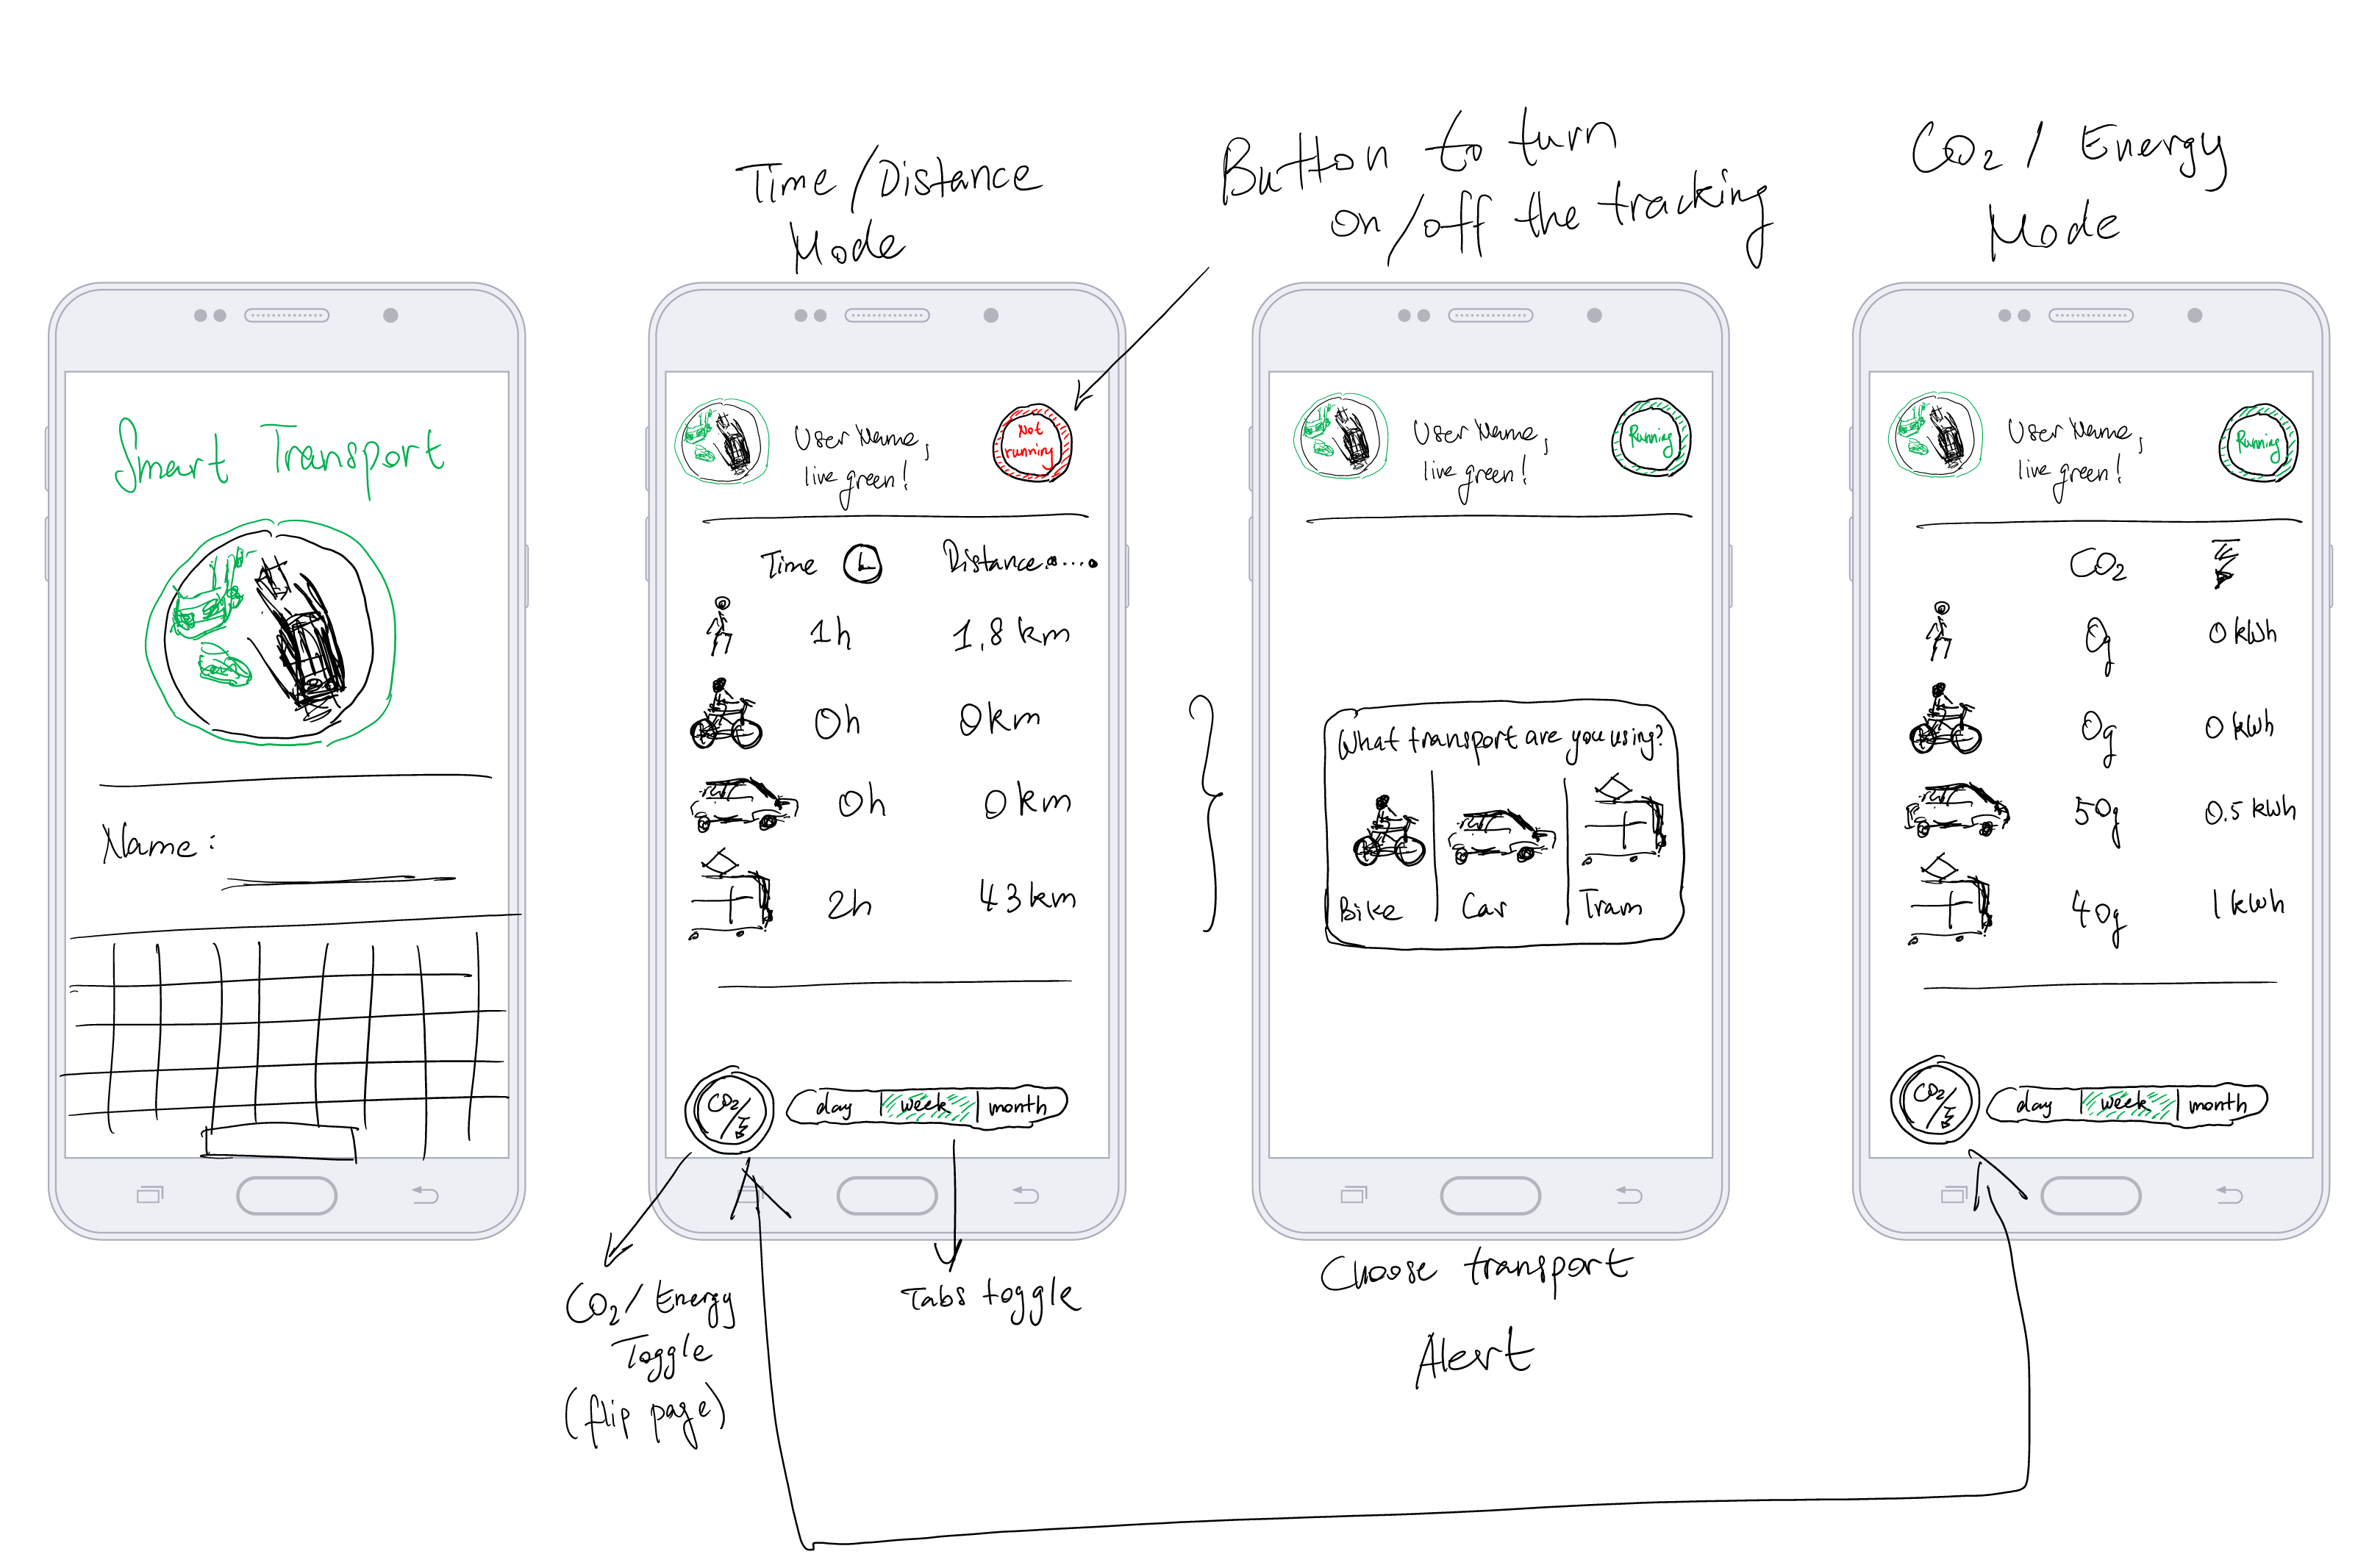
\includegraphics[width=\columnwidth]{ressources/mock-up.png}
	\vspace{-1.5em} % use negative white space to fix too large gaps
	\caption{Mock-Up of Smart Transport}
	\label{fig:mock-up}
\end{figure}


\subsection{Tracking the User}

One of the first problems we faced when developing this app was figuring out how we were going to track the user’s movement. It was clear to us that an automation of this process was necessary, since allowing the user to input information about his or her transportation, would be too time consuming. Luckily, the vast majority of today’s phones has an embedded global positioning system, which could help us determine the route, distance and speed of whatever trip the user is conducting.

\subsection{Database}

To get the GPS benefits described above we would frequently have to store the current position, and here we decided to use the embedded SQL database engine; SQLite. No server is involved in our application, so the data is simply stored locally in a database in the file system.

\subsection{Automatically Infer Means of Transport}

If we decided to let the user input his or her means of transport manually, the backend side would be done here. However, this is also not very user friendly, as it would take up too much time for the average user. We would have to make our application automatically determine the transportation means of the user for it to become usable. Lots of ideas were discussed here on how to determine means of transport, ranging from simple to advanced solutions.

First off, we could easily guess that the user is in a vehicle of some kind, just by checking if the average travelling speed is exceeding a certain threshold.
Adding to this we could analyse the flow of the transportation. This included parameters such as number of stops, top speed and average speed. This could help us determine if the passenger is travelling by bike – few and very short stops, and not very high top speed, all relative to other means of transport in the system. Top speed and average speed could also help us determine if user is a passenger in a train or bus/tram.
We used Google’s Activity Detection API to help us determine whether the user is in a vehicle, running, walking or standing still. Moreover, it also gives back a confidence level, how likely it is that the activity is correct with a number between 1-100. By implementing this, and continuously storing the result in a database, we can then analyse the pattern that occurs in different means of transport.


\subsection{Analysing Result from Different Means of Transport}

When going out in Zurich we tested different means of transport, we noticed different pattern in the data that we continuously collected in our database. Most importantly, we took a closer look at the speed, and how long the vehicle stood still as well as how often that happened. 

We surmised that the solution described above would be difficult to make, so that it always gives very accurate results. One type of vehicle pattern could look very similar another in certain circumstances. A better way would be to use an API from SBB, where one can see what type of transportation means  should be at a particular position at a certain time. However, we decided that would take too long to fit the time frame for this project.


\subsection{Graphical User Interface}

After starting up the app for the first time, the user will be asked for her name, simply for it to feel more interactive which is displayed in figure~\ref{fig:login} and to later be able to display the result in a more personal way.
We decided to display information about the CO2 emissions and energy usage in a table-like form, which can be seen in figure. The user is then able to toggle between time/distance and CO2/energy.

\begin{figure}[h]
	\centering
	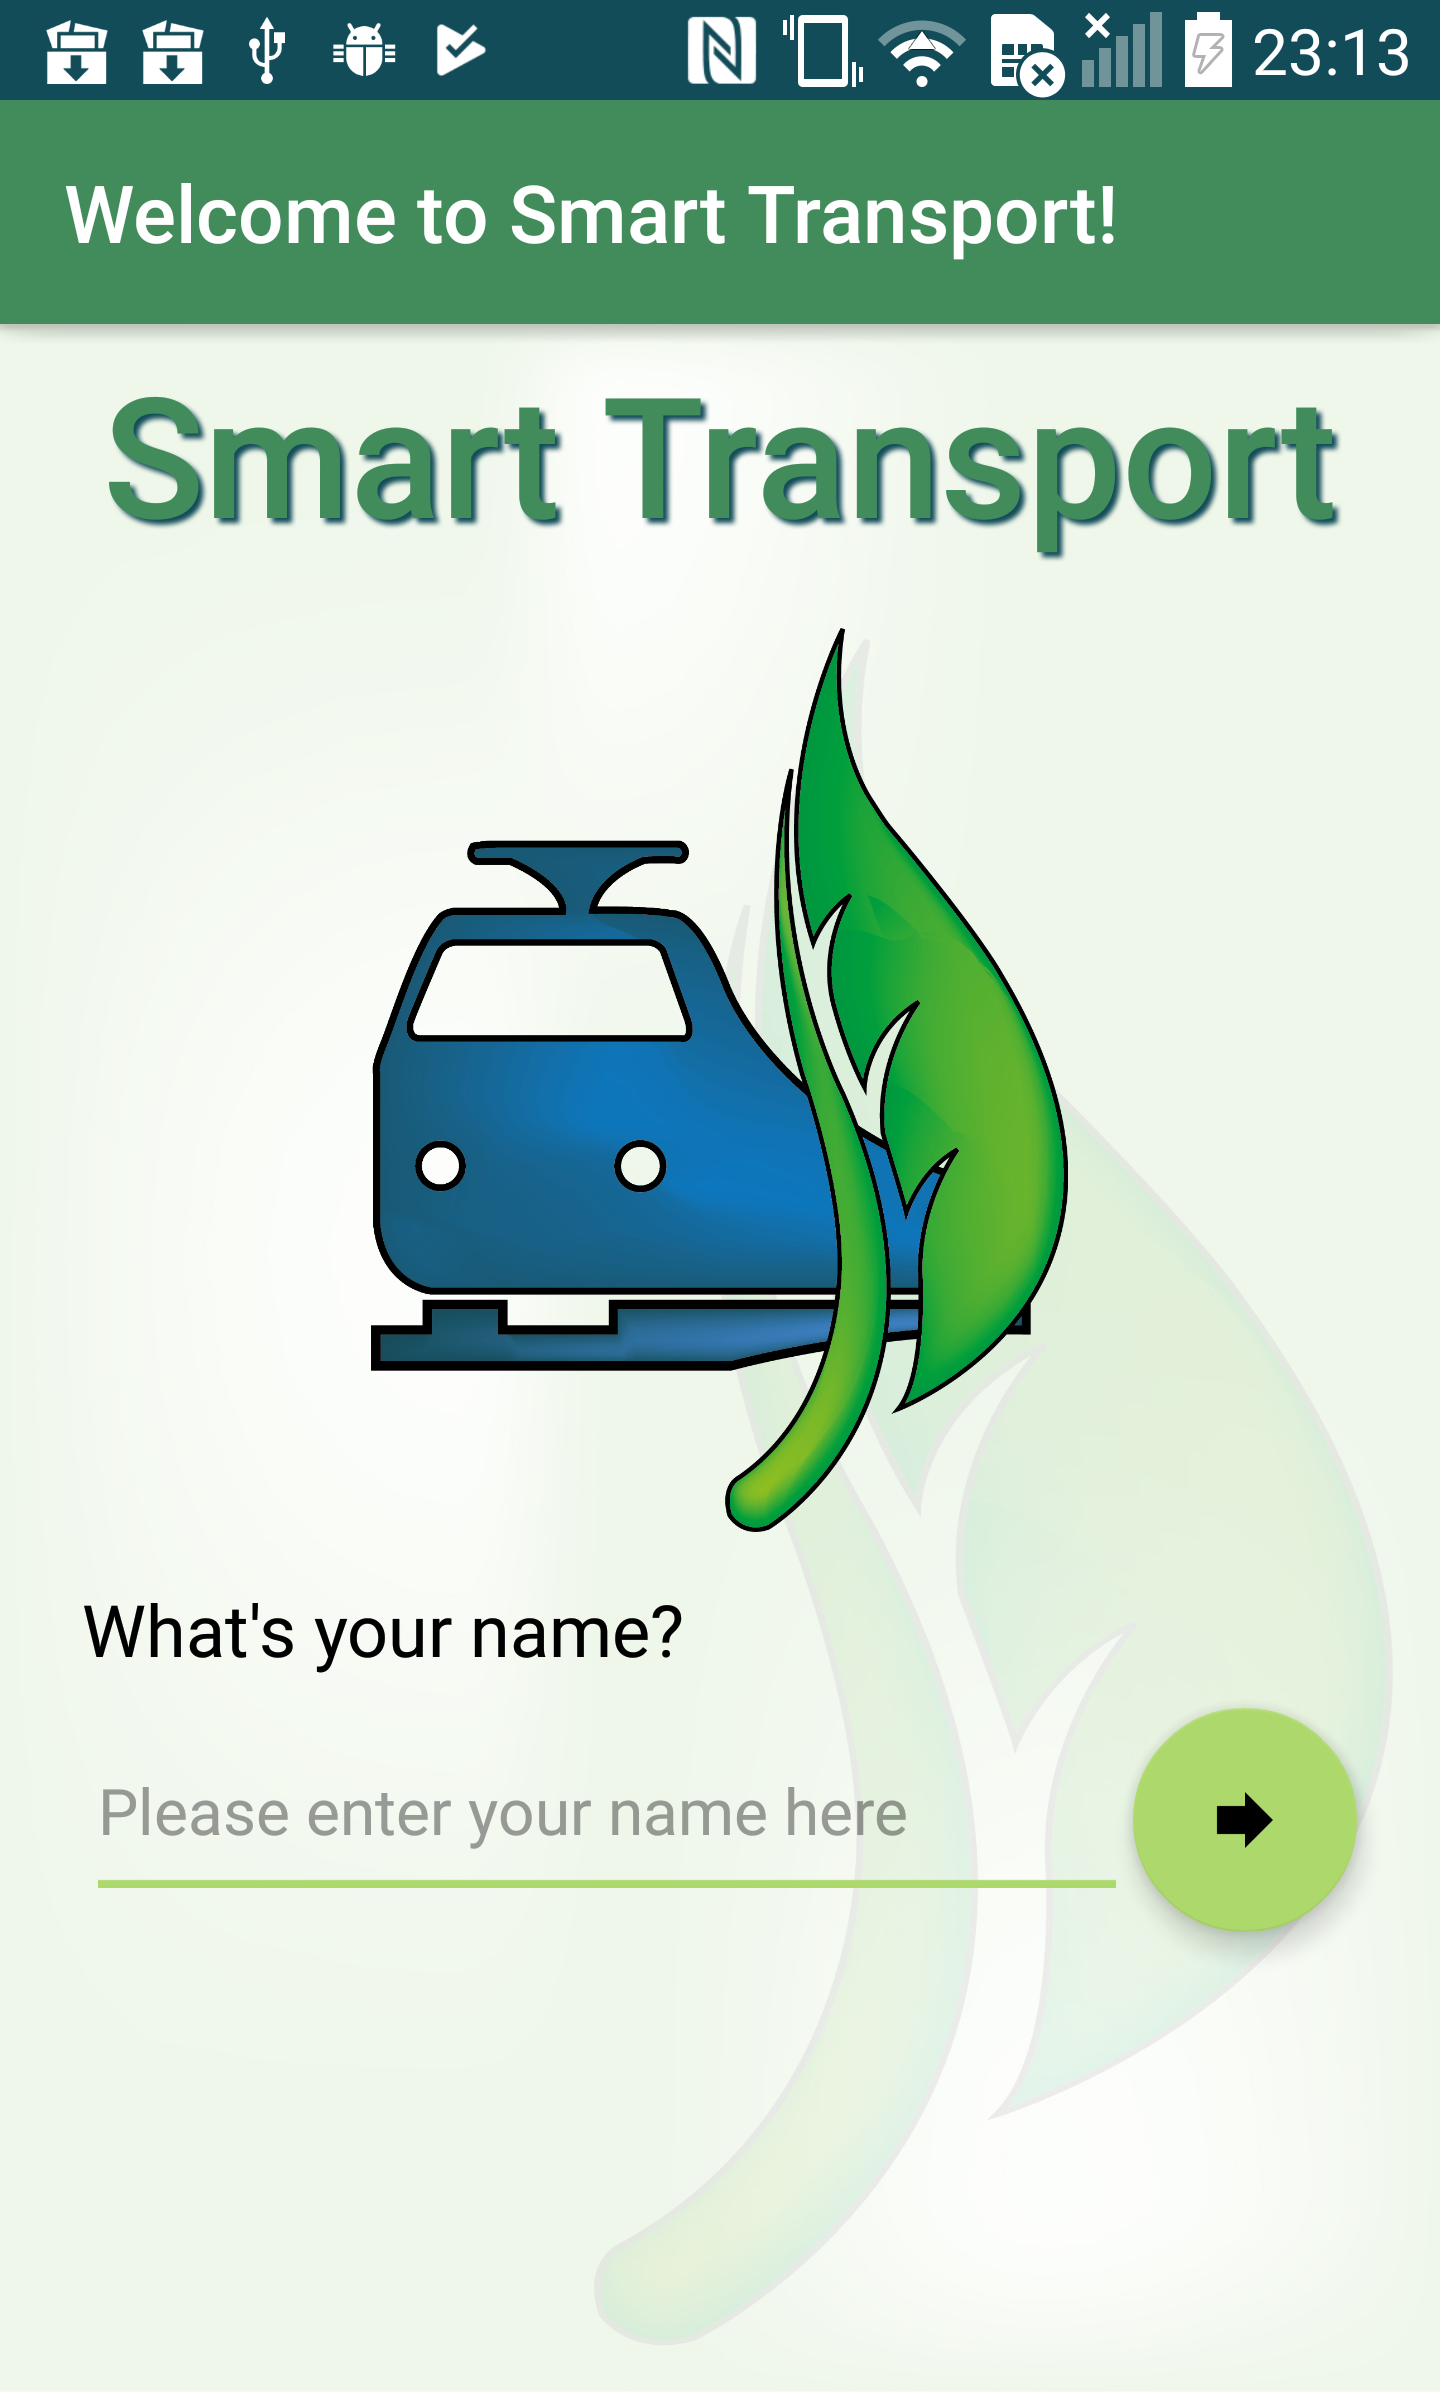
\includegraphics[width=\columnwidth, height=6cm, keepaspectratio]{ressources/LoginActivity.png}
	\vspace{0em} % use negative white space to fix too large gaps
	\caption{Login Activity with Question}
	\label{fig:login}
\end{figure}

\begin{figure}[h]
	\centering
	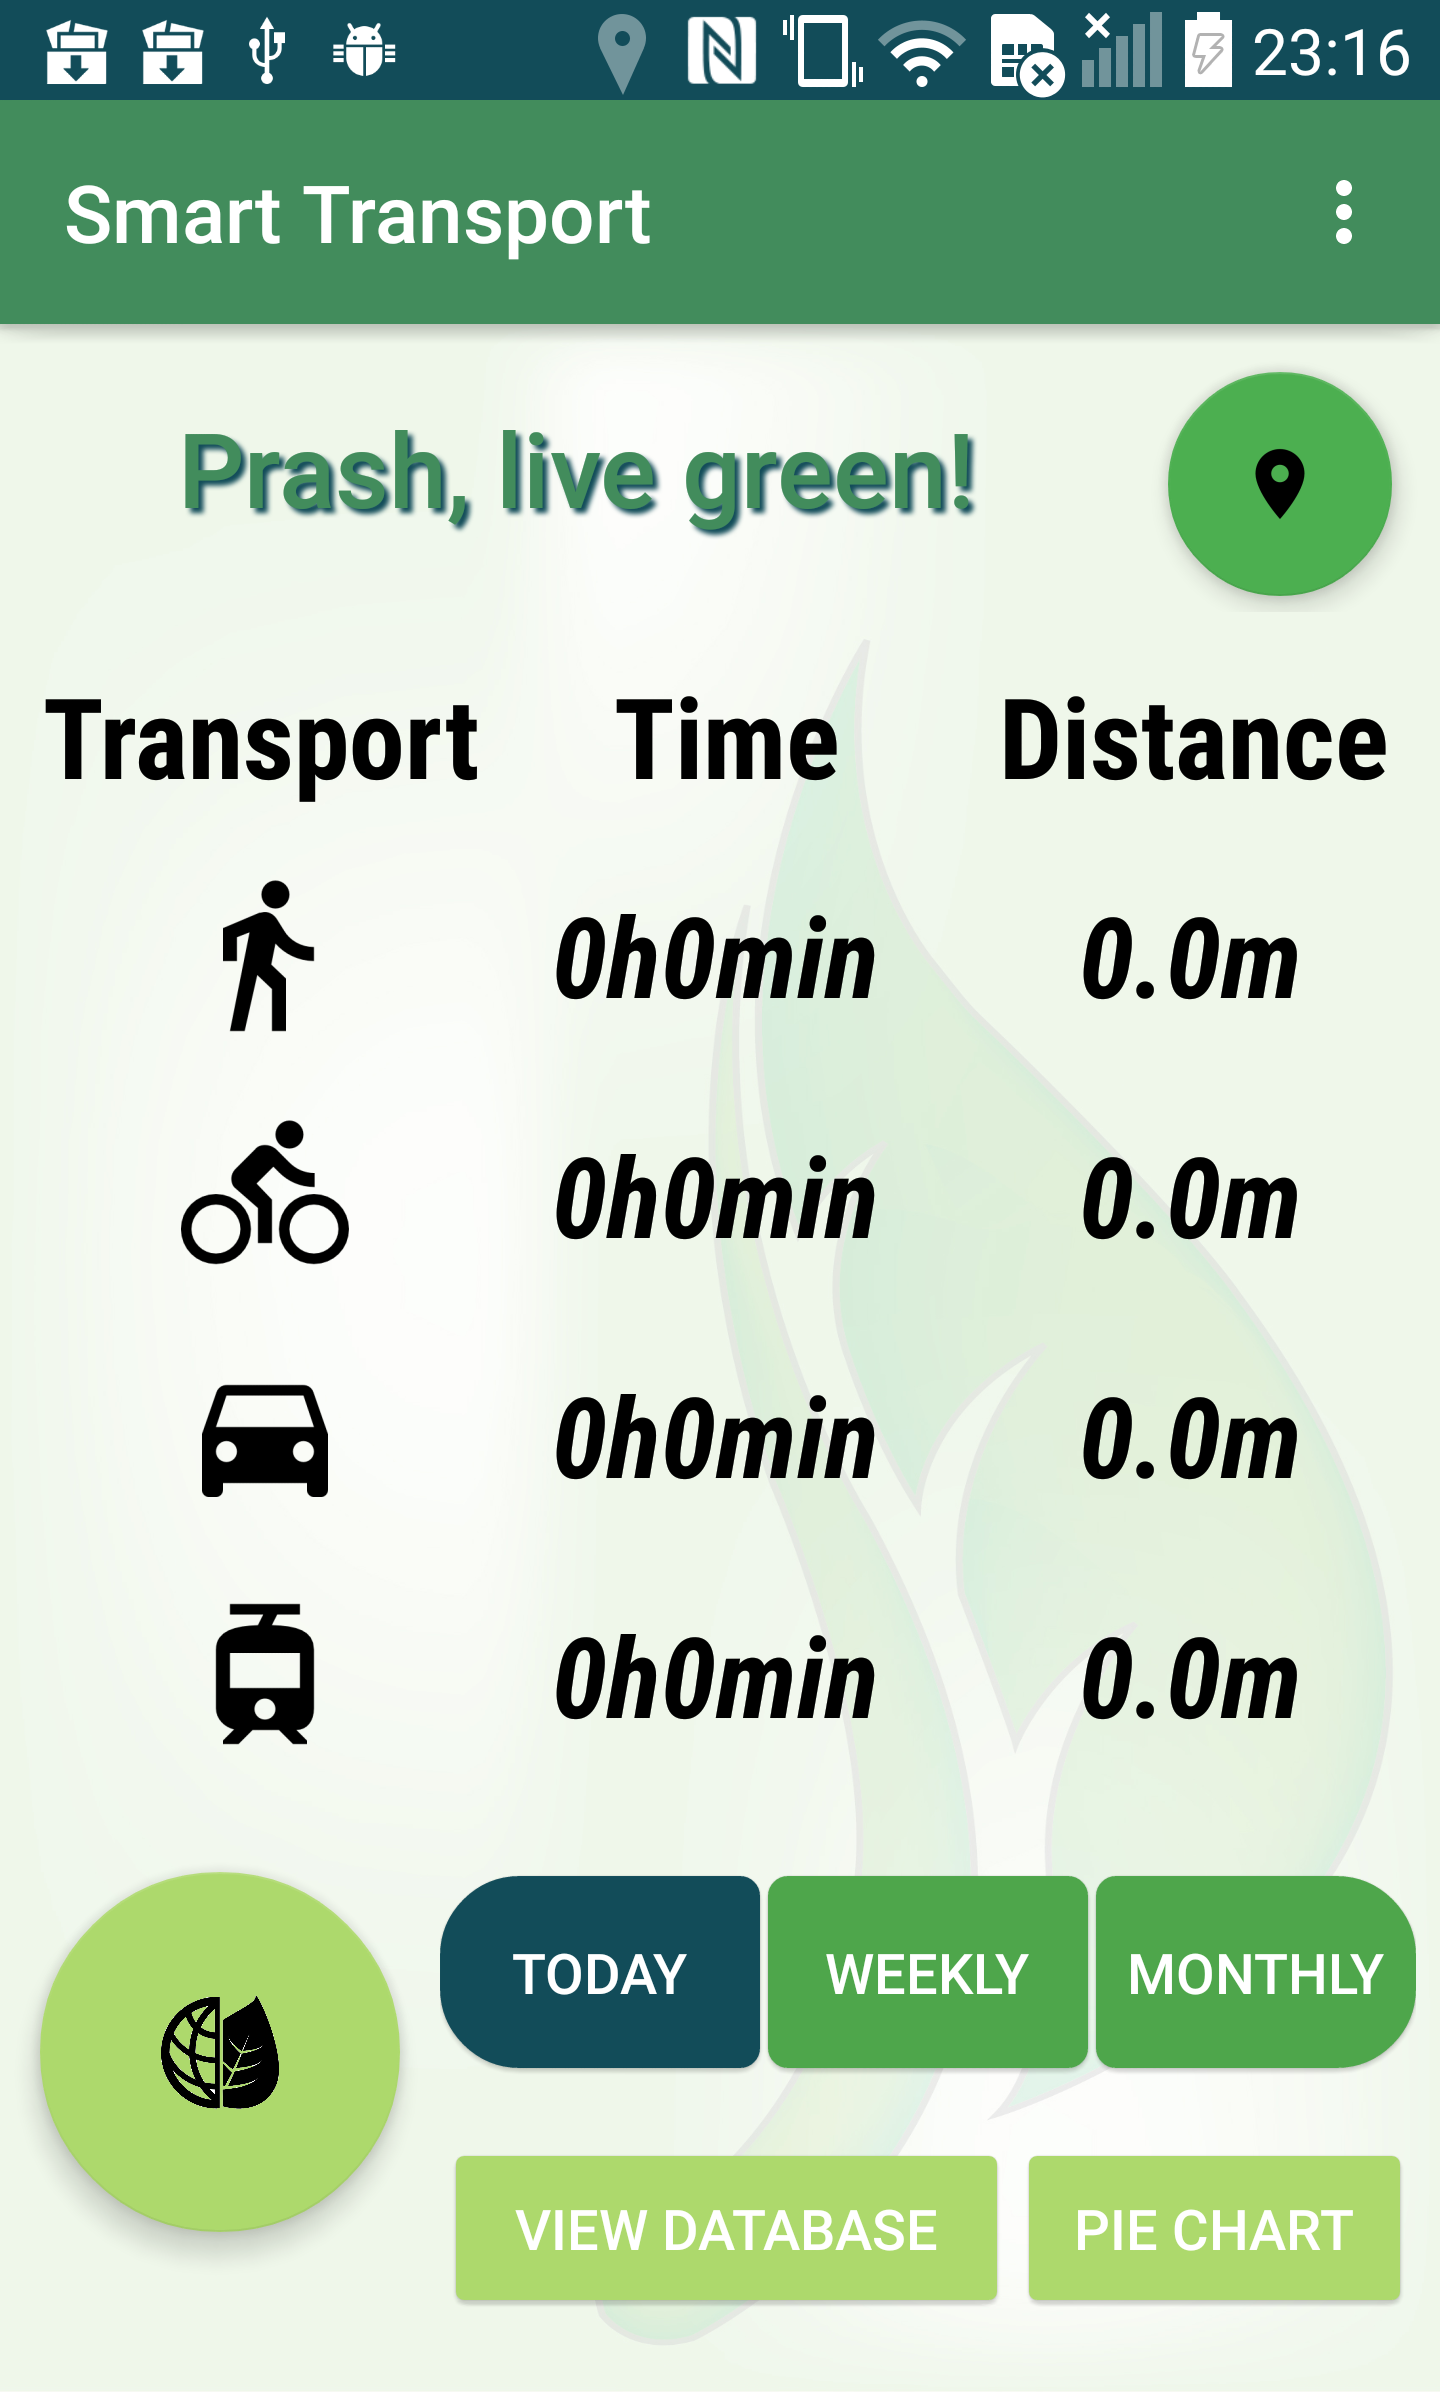
\includegraphics[width=\columnwidth, height=6cm, keepaspectratio]{ressources/MainActivityOn.png}
	\vspace{0em} % use negative white space to fix too large gaps
	\caption{Main Activity with Table}
	\label{fig:main}
\end{figure}


\subsection{Material for Calculating CO2 Emissions and Energy Usage}

The energy usage and CO2 emissions from different vehicles varies a lot depending on the model. With this in mind, we wanted the results generated to be as accurate as possible for travel within Switzerland first and foremost. We found a table in a report by SBB covering the averages of both CO2 emissions and primary energy usage, for all different means of transport in SBB’s network, in passenger kilometres~\cite{sbbcalculator2017}.

It is worth adding here, that it was no coincidence that we chose to use the primary energy per passenger kilometre (pkm). The alternative would have been to use final energy pkm, however, that would in our opinion have misled the user about his or her real ecological footprint. Of course, final energy better reflects the amount of energy consumed, nevertheless following that energy back to how it was generated better reflects reality. Only then it is actually fair to compare, for example, a car ride to an activity such as walking. 
Furthermore, we did not think our user would be able to relate to ml gasoline/pkm, and chose to convert it to Mega Joule. 


\subsection{Summary of Architecture}

The MainActivity class of the application runs on the UI thread while location/speed updates and Activity Detection run on separate threads in the background. Both of these are enabled/disabled through the toggle button on the top right corner of the main screen. All activities are accumulated and stored in an SQLite database locally on the phone. The frequency of location updates by default is 10ms and can be adjusted from the Settings screen accessible through the MainActivity. Increasing this value means better performance, however can lead to misclassifications of the car/tram classification. An aggregation of the time spent in each mode of transport is displayed as a pie chart upon launching the PieChart activity from the MainActivity. An interface that holds SQL Query constants assists in fetching data.

The logic for differentiating between tram/car is as follows:

After experimentation we were able to observe that while travelling on a tram, the recordedActivities database exhibits a certain pattern of “blocks” of “Standing Still” followed by “In Vehicle” and the maximum speed detected in a tram was approximately 60km/h. Thus, to differentiate between a tram and a car, we take two factors into account - namely the “blocks” pattern and the average speed over these blocks compared to the current speed. To account for experimental error, we also define a tolerance percentage. This parameter can be fine tuned for better differentiation depending on the situation.

Integrating google maps for this differentiation is an option but the tradeoffs are similar and the accuracy one can expect from using maps or our method are comparable. For example, a naive method would be checking if the travelled route coincides with a tram route and coincidentally a vehicle could also be moving along such a route, leading to misclassification. After this analysis we decided to provide parameters to the user to adjust and fine tune the accuracy of differentiation.

\section{Summary and Conclusions}

The biggest challenge in this project was making educated guesses about the means of transport while ensuring that these tasks happen on a separate background thread that can be enabled or disabled by the user. Additionally we ensured that this code could be extended in the future with easy by writing modular code with clean, separated interfaces. With the addition of storing everything in an SQLite Database, this can be used for several extensions or more in depth data analysis to provide meaningful feedback to the user. For example, we integrated a pie chart into the UI to display the breakdown of travel modes, and this can be extended to provide information such as breakdown for a particular part of the day that can be potentially be optimized to reduce one's’ CO2 footprint.


\bibliographystyle{IEEEtran}
\bibliography{smart-energy-literature}

\clearpage

\end{document}
